\part{Synchronous machine}
\title[Synchronous machine]{Synchronous machine}  
\date{}  
\frame{\titlepage} 

%%%%%%%%%%%%%%%%%%%%%%%%%%%%%%%%%%%%%%%%%%%%%%%%%%%%%%%%%%%%%
%% Synchronous machine (SM) rotor types %%
%%%%%%%%%%%%%%%%%%%%%%%%%%%%%%%%%%%%%%%%%%%%%%%%%%%%%%%%%%%%%
\begin{frame}
	\frametitle{Synchronous machine (SM) rotor types}
	\begin{figure}
		\centering
		\begin{subfigure}{0.49\textwidth}
			\centering
			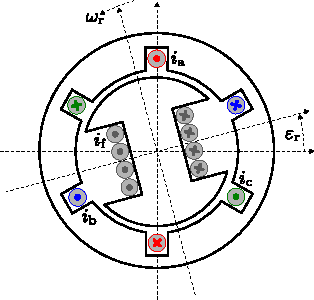
\includegraphics[width=0.8\textwidth]{fig/lec07/SM_salient_pole.pdf}
			\caption{Salient pole rotor}
		\end{subfigure}
		\hfill
		\begin{subfigure}{0.49\textwidth}
			\centering
			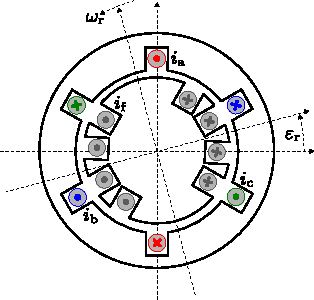
\includegraphics[width=0.8\textwidth]{fig/lec07/SM_cylindrical_rotor.pdf}
			\caption{Cylindrical rotor}
		\end{subfigure}
        \caption{Major rotor types of synchronous machines (SM)} 
        \label{fig:examples_SM_rotor}
	\end{figure}
\end{frame}

%%%%%%%%%%%%%%%%%%%%%%%%%%%%%%%%%%%%%%%%%%%%%%%%%%%%%%%%%%%%%
%% SM application examples %%
%%%%%%%%%%%%%%%%%%%%%%%%%%%%%%%%%%%%%%%%%%%%%%%%%%%%%%%%%%%%%
\begin{frame}
	\frametitle{SM application examples}
	\begin{figure}
		\centering
		\begin{subfigure}{0.49\textwidth}
			\centering
			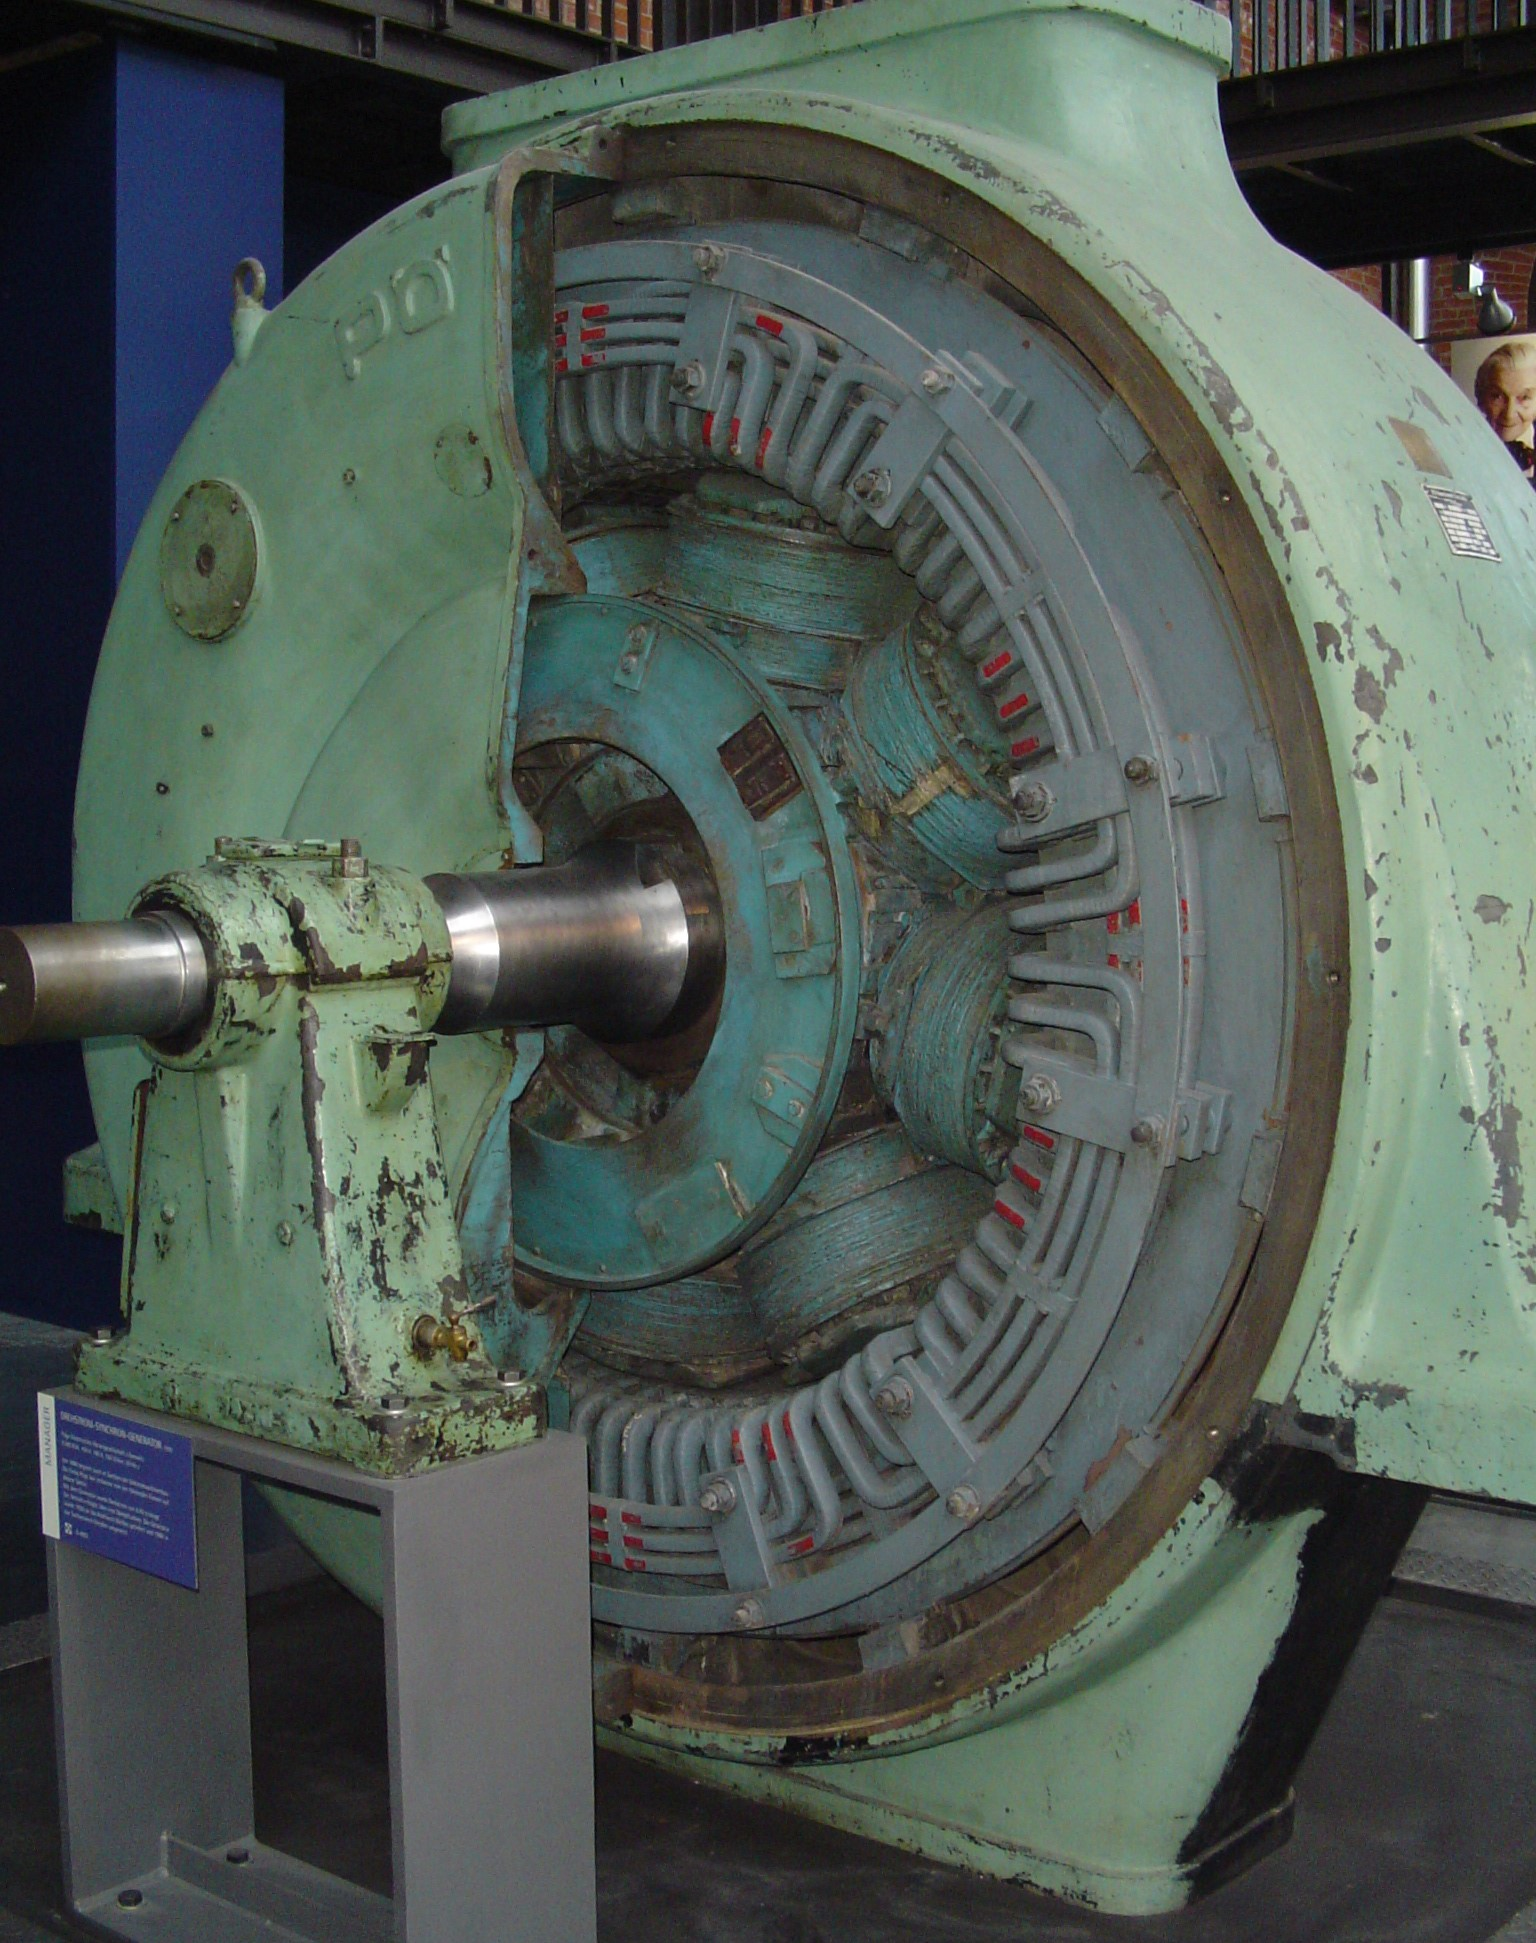
\includegraphics[height=0.55\textheight]{fig/lec07/Salient_pole_rotor.jpg}
			\caption{\SI{2}{\mega\volt\ampere} generator from 1920 (source: \href{hhttps://commons.wikimedia.org/wiki/File:Drehstrom-Synchron-Generator.jpg}{Wikimedia Commons}, Kolossos, \href{https://creativecommons.org/licenses/by-sa/3.0/deed}{CC BY-SA 3.0})}
		\end{subfigure}
		\hfill
		\begin{subfigure}{0.49\textwidth}
			\centering
			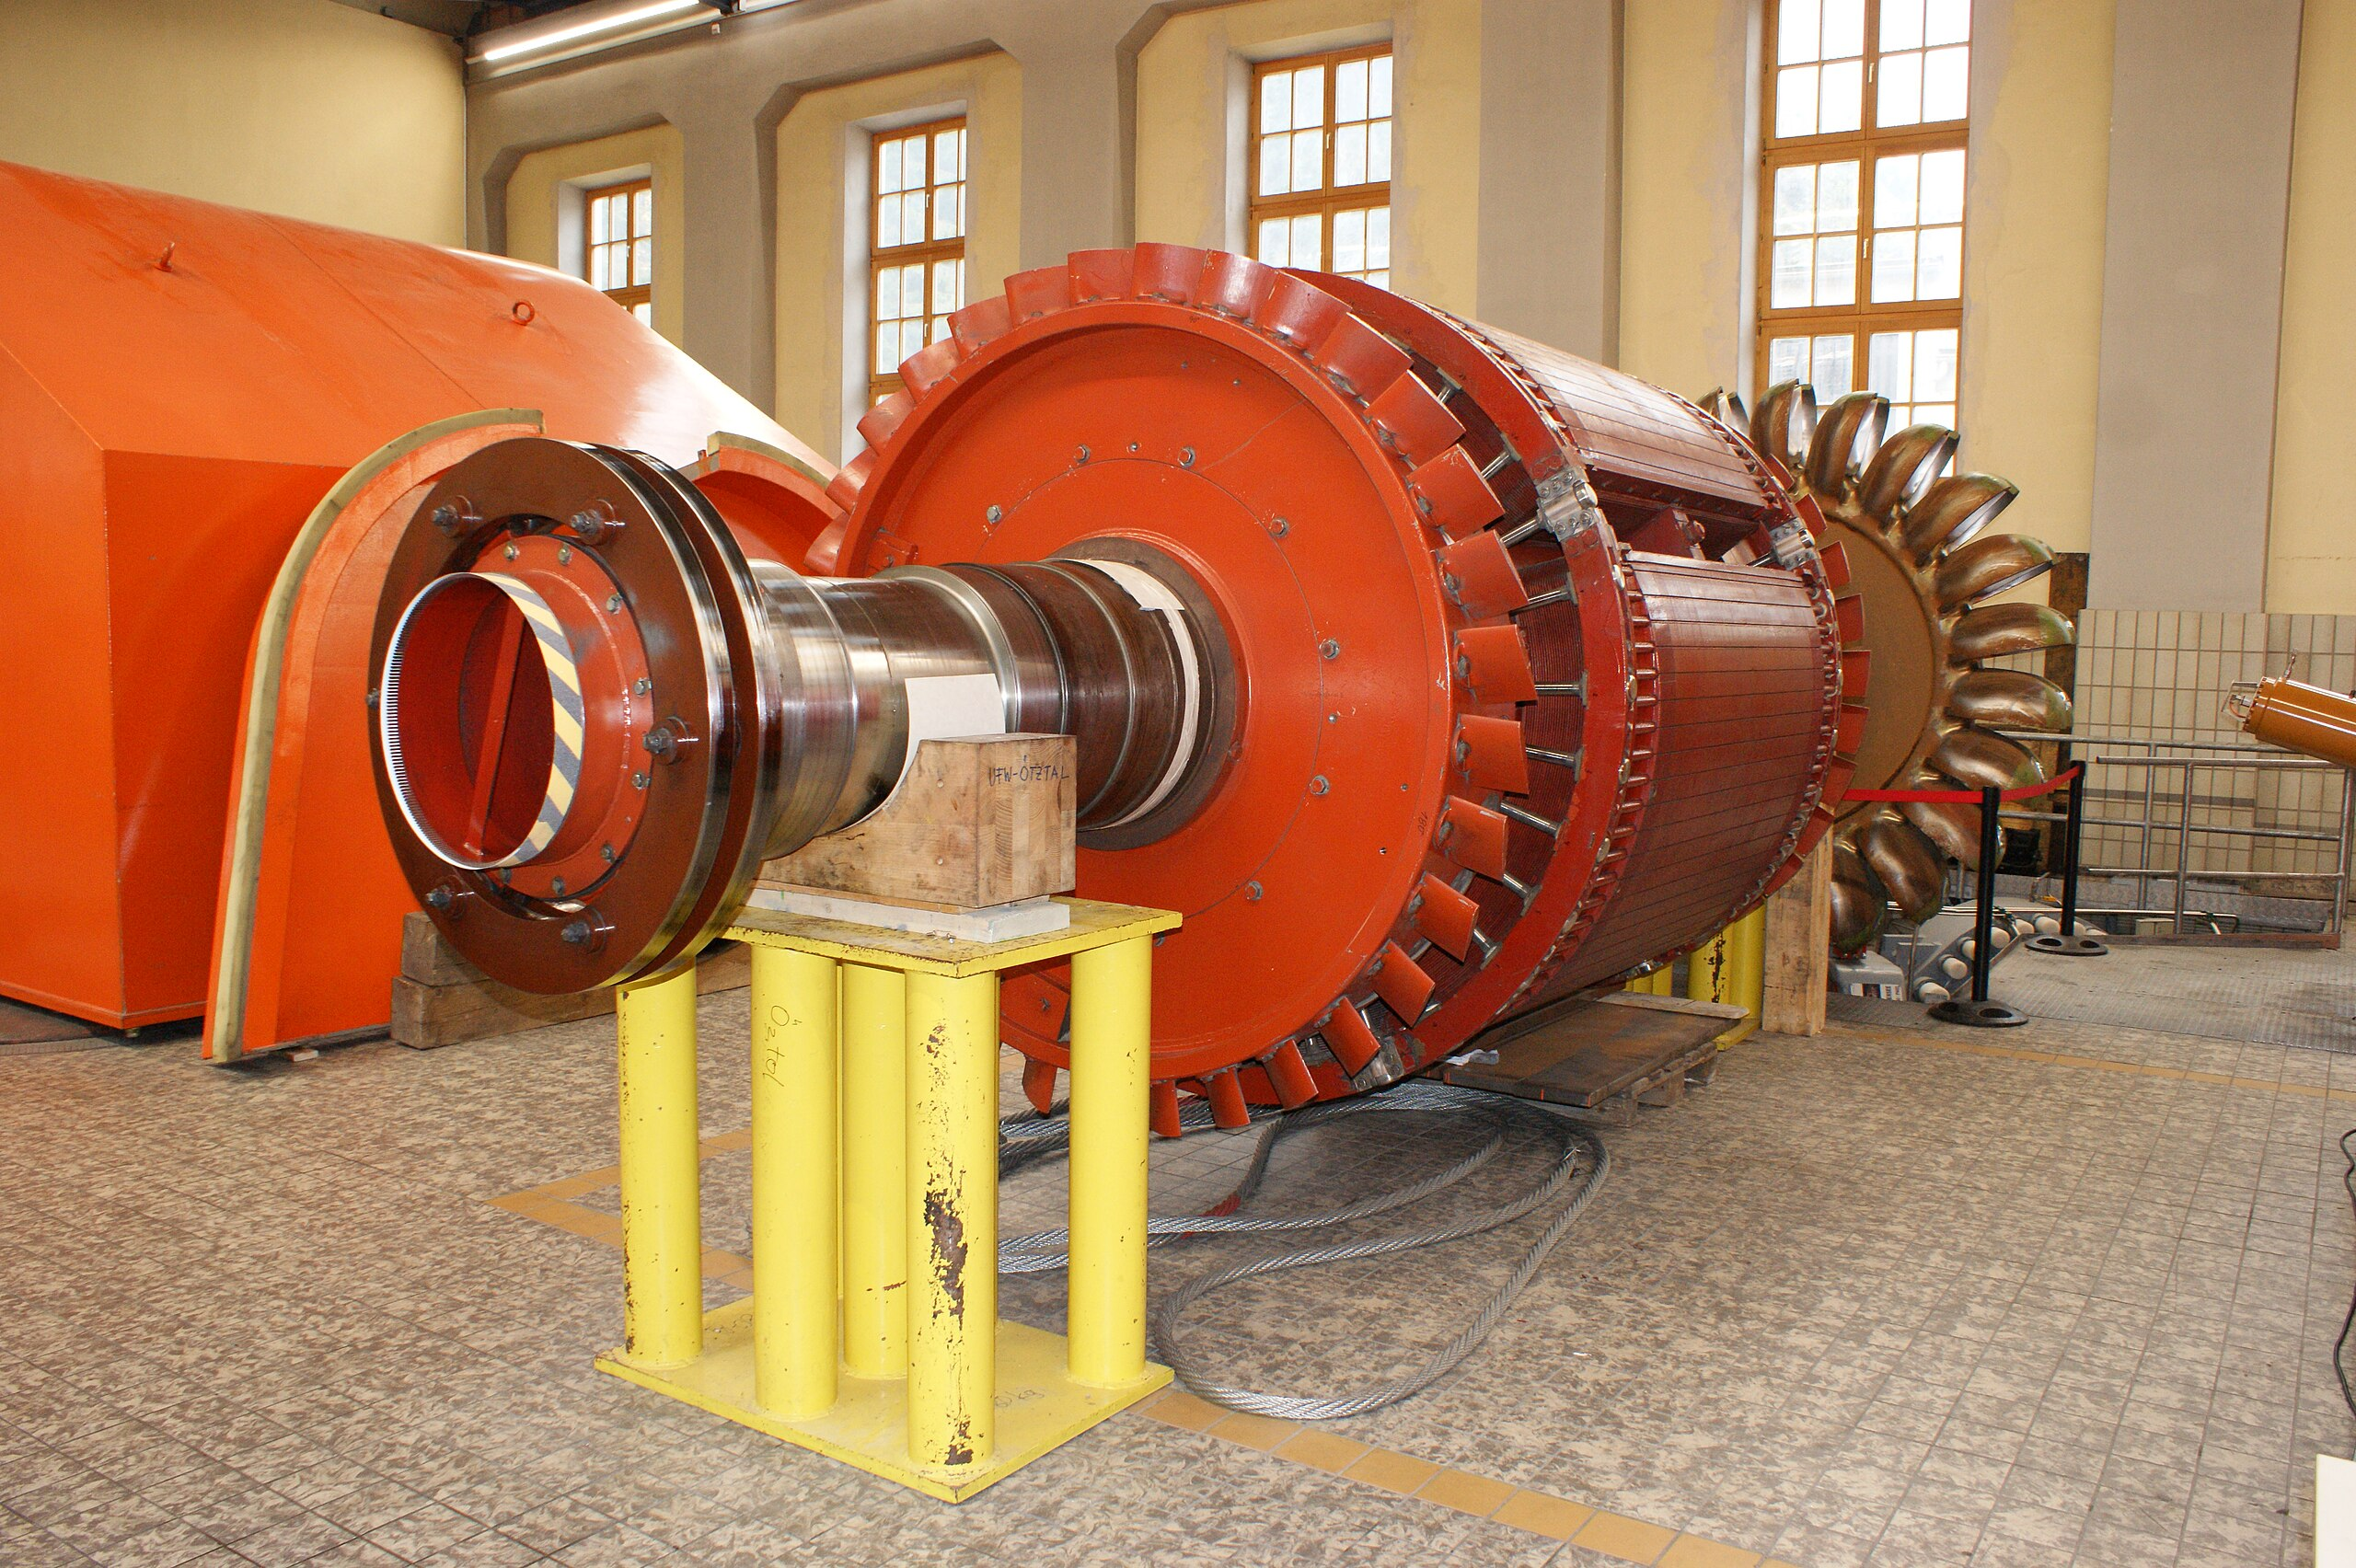
\includegraphics[height=0.55\textheight]{fig/lec07/Pelton_wheel_rotor.jpg}
			\caption{\SI[tight-spacing=true]{36}{\mega\volt\ampere} Pelton wheel generator (source: \href{https://commons.wikimedia.org/wiki/File:Wald_am_Arlberg-OeBB_Spullersee_power_plant-M1-Rotor-09ASD.jpg}{Wikimedia Commons},  	Asurnipal, \href{https://creativecommons.org/licenses/by-sa/4.0/deed}{CC BY-SA 4.0})} 
		\end{subfigure}
        \caption{SM examples with salient pole rotor type} 
        \label{fig:examples_SM_applications_01}
	\end{figure}
\end{frame}

%%%%%%%%%%%%%%%%%%%%%%%%%%%%%%%%%%%%%%%%%%%%%%%%%%%%%%%%%%%%%
%% SM application examples (cont.) %%
%%%%%%%%%%%%%%%%%%%%%%%%%%%%%%%%%%%%%%%%%%%%%%%%%%%%%%%%%%%%%
\begin{frame}
	\frametitle{SM application examples (cont.)}
	\begin{figure}
		\centering
		\begin{subfigure}{0.49\textwidth}
			\centering
			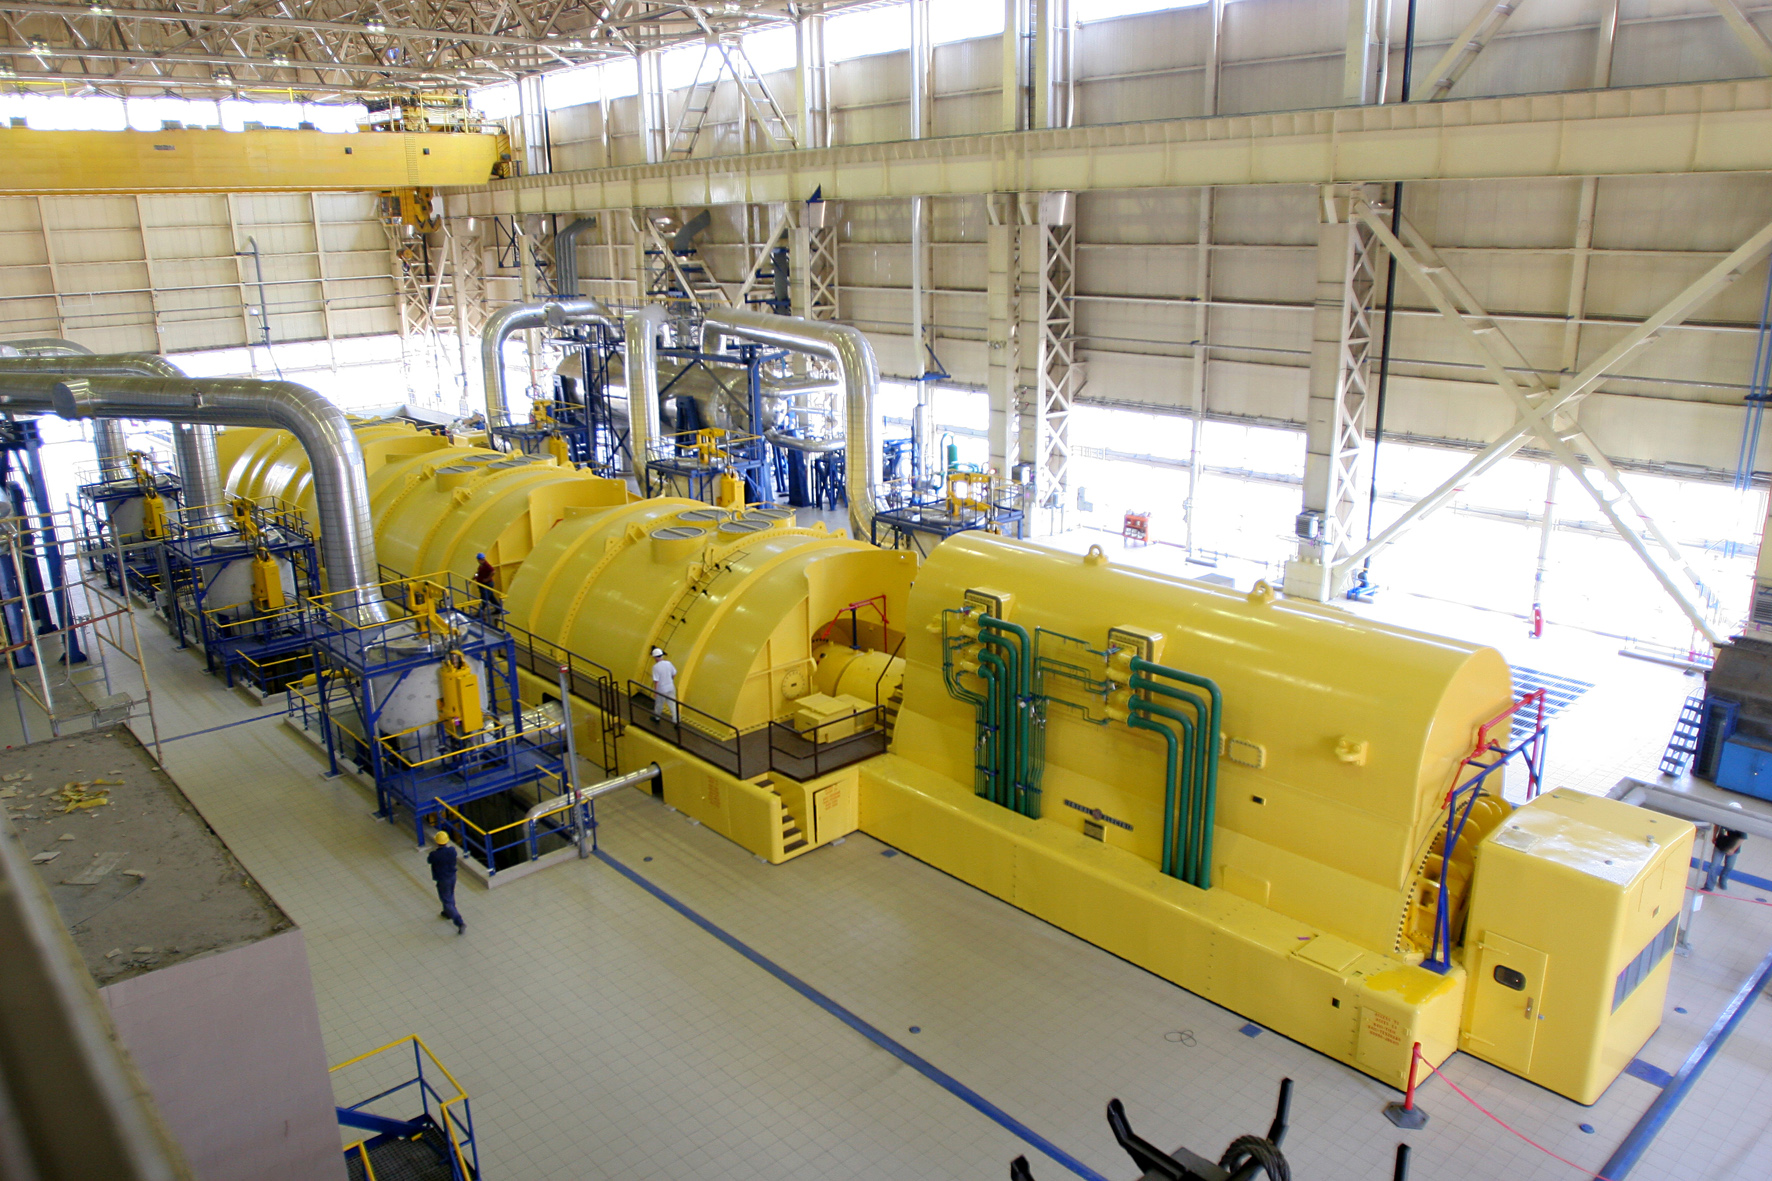
\includegraphics[height=0.55\textheight]{fig/lec07/Turbogenerator.jpg}
			\caption{\SI{650}{\mega\volt\ampere} turbogenerator from Cernavodă nuclear power plant (source: \href{https://commons.wikimedia.org/wiki/File:Grupul_turbogenerator_CNE_Cernavoda.jpg}{Wikimedia Commons}, R. Lavinia, \href{https://creativecommons.org/licenses/by-sa/4.0/deed}{CC BY-SA 4.0})}
		\end{subfigure}
		\hfill
		\begin{subfigure}{0.49\textwidth}
			\centering
			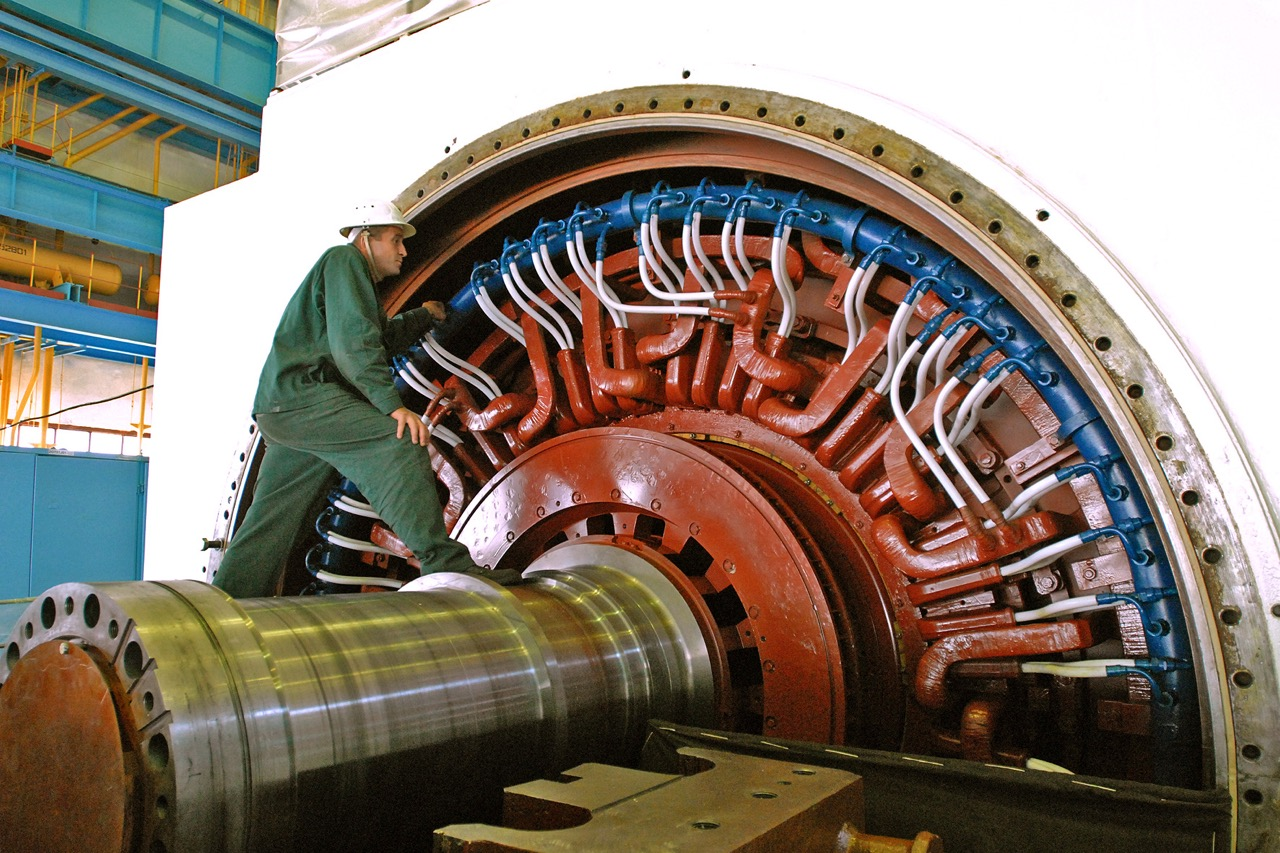
\includegraphics[height=0.55\textheight]{fig/lec07/Turbogenerator_rotor.jpg}
			\caption{\SI[tight-spacing=true]{1}{\giga\volt\ampere} turbogenerator SM rotor from Balakovo nuclear power plant (source: \href{https://commons.wikimedia.org/wiki/File:BalakovoNPP_tb.jpg}{Wikimedia Commons},  A. Seetenky, \href{https://creativecommons.org/licenses/by-sa/3.0/deed}{CC BY-SA 3.0})} 
		\end{subfigure}
        \caption{SM examples with cylindrical rotor type} 
        \label{fig:examples_SM_applications_02}
	\end{figure}
\end{frame}

%%%%%%%%%%%%%%%%%%%%%%%%%%%%%%%%%%%%%%%%%%%%%%%%%%%%%%%%%%%%%
%% Visualization of the synchronous machine operation %%
%%%%%%%%%%%%%%%%%%%%%%%%%%%%%%%%%%%%%%%%%%%%%%%%%%%%%%%%%%%%%
\begin{frame}
	\frametitle{Visualization of the synchronous machine operation}
    \vspace{-0.275cm}
    \begin{figure}
        \centering
        \movie{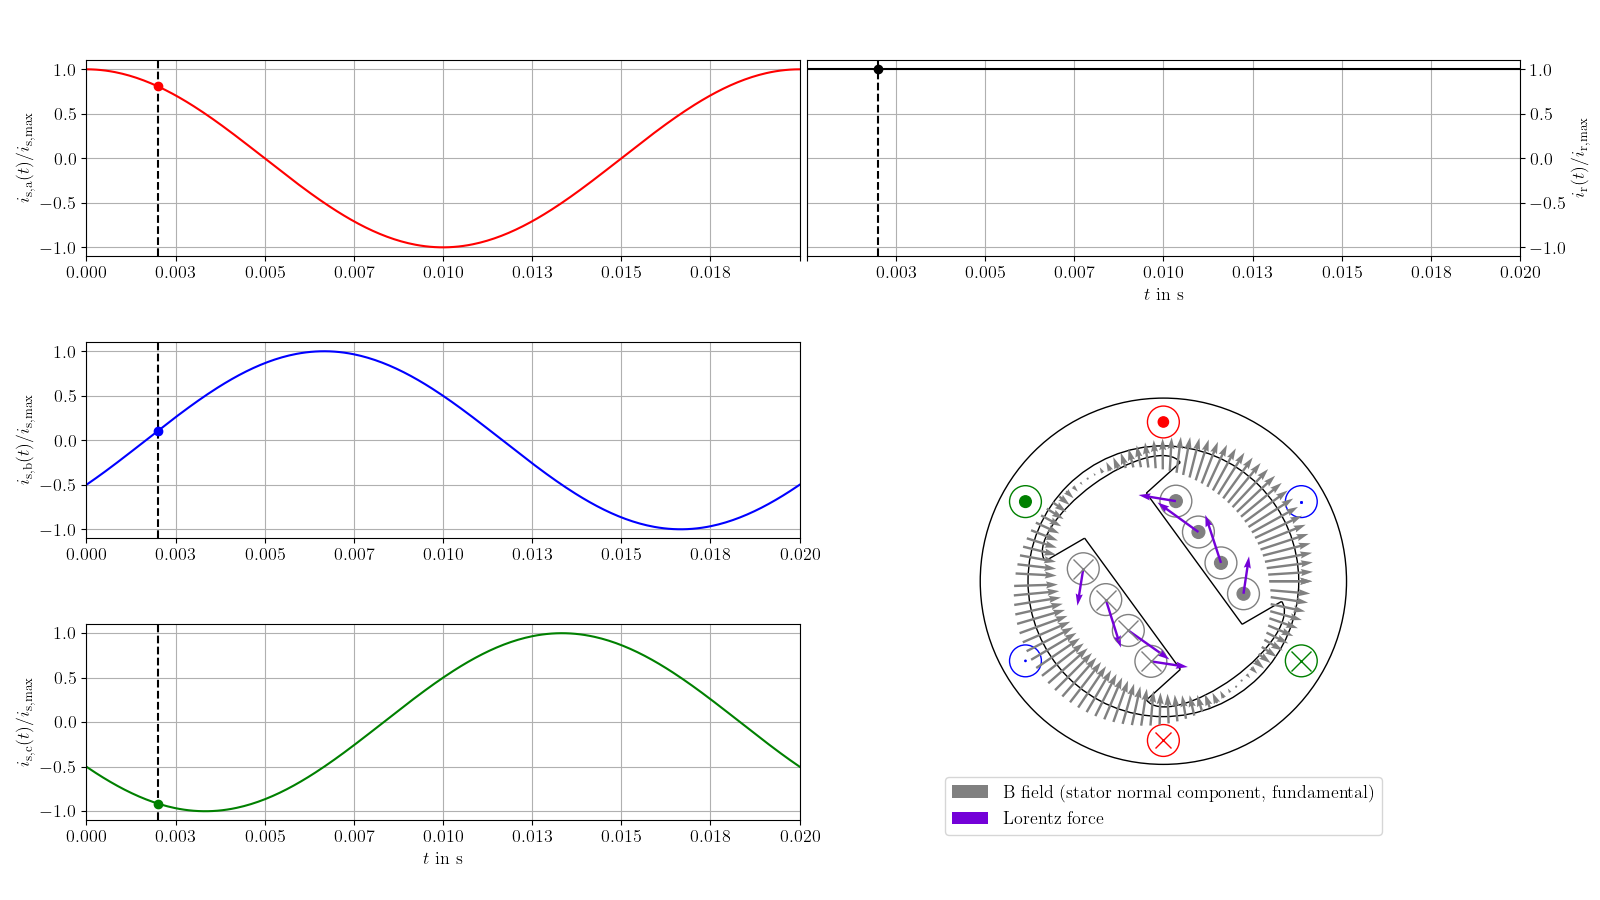
\includegraphics[height=0.85\textheight]{fig/lec07/SM_load_angle_90_preview.png}}{fig/lec07/SM_load_angle_90_animation.gif}
        \vspace{-0.25cm}
        \caption{Exemplary SM operation at $\omega=2 \pi \SI{50}{\per\second}$ in motoric operation (positive average torque)}
        \label{fig:SM_load_angle_90_animation}
    \end{figure}
\end{frame}

%%%%%%%%%%%%%%%%%%%%%%%%%%%%%%%%%%%%%%%%%%%%%%%%%%%%%%%%%%%%%
%% Visualization of the synchronous machine operation (cont.) %%
%%%%%%%%%%%%%%%%%%%%%%%%%%%%%%%%%%%%%%%%%%%%%%%%%%%%%%%%%%%%%
\begin{frame}
	\frametitle{Visualization of the synchronous machine operation (cont.)}
    \vspace{-0.275cm}
    \begin{figure}
        \centering
        \movie{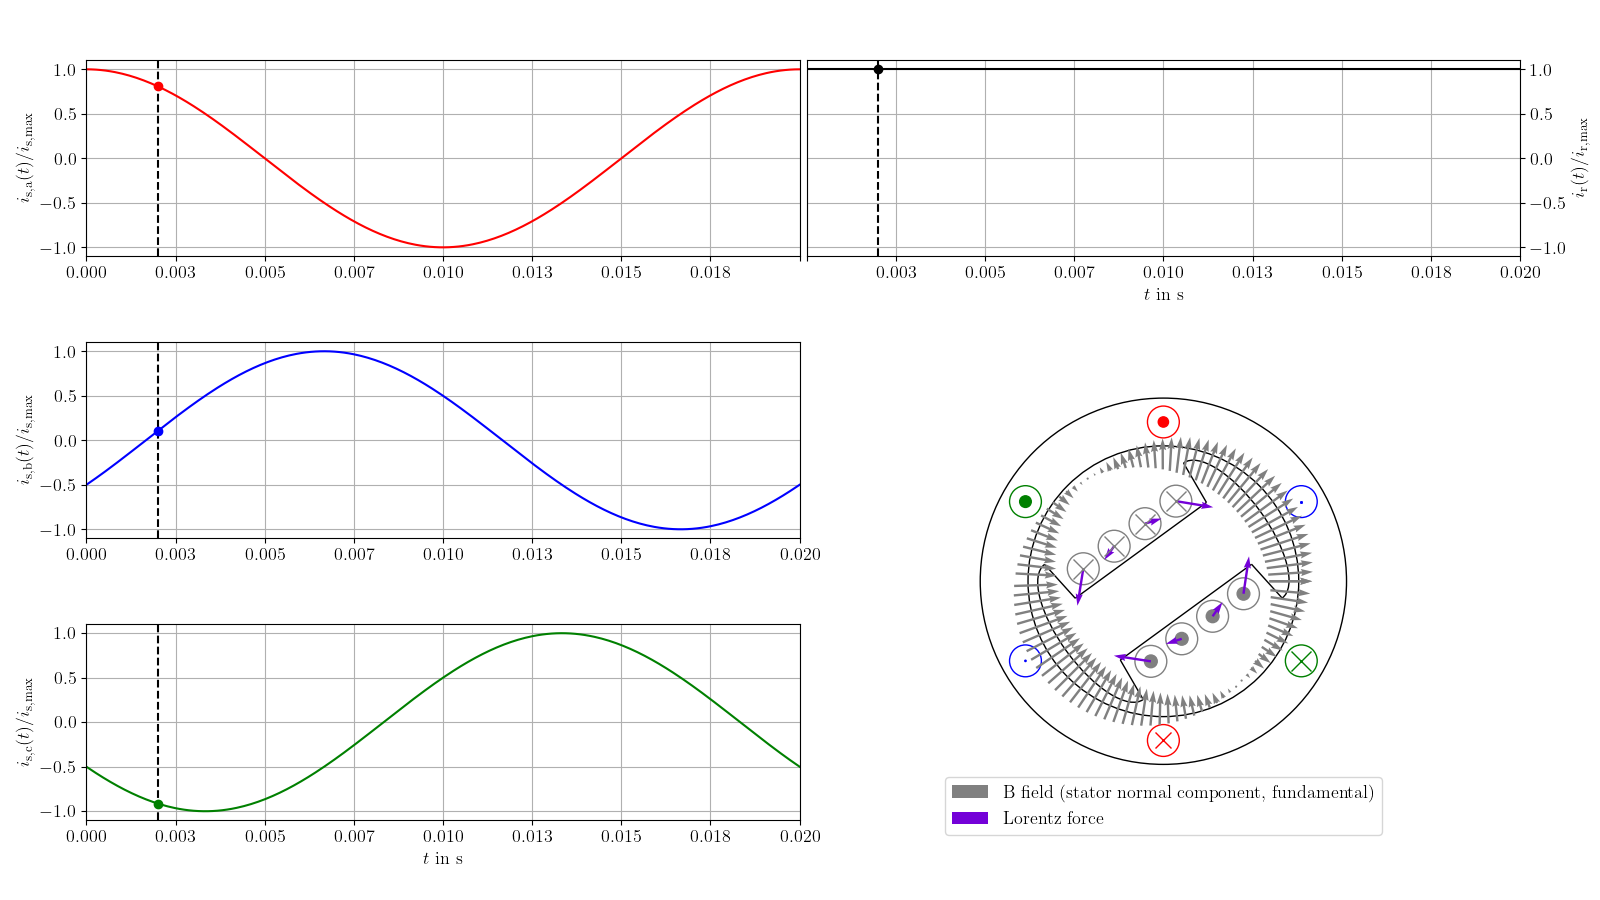
\includegraphics[height=0.85\textheight]{fig/lec07/SM_load_angle_0_preview.png}}{fig/lec07/SM_load_angle_0_animation.gif}
        \vspace{-0.25cm}
        \caption{Exemplary SM operation at $\omega=2 \pi \SI{50}{\per\second}$ in no-load operation (zero average torque)}
        \label{fig:SM_load_angle_0_animation}
    \end{figure}
\end{frame}